\documentclass{ximera}

\title{Optimization Activity Facilitator Guide}
\author{MATH 425: Calculus I}

\begin{document}
\begin{abstract}
    Working with the peers in your group, solve the following problems. Make sure to show and justify all your work. Make sure everyone in the group understands the solution and participates. Be prepared to report your answers to the whole class. 
\end{abstract}
\maketitle

\textbf{Student Learning Objectives}
Students will be able to:
\begin{itemize}
    \item Set up optimization problems involving geometric areas and volumes.
    \item Create objective functions for optimization based on given geometric area and volumes and/or other constraints.
\end{itemize}

\textbf{Prerequisite Knowledge:} This activity is meant to be used after Optimization is covered in class. Students will need to understand how to take the derivative and find critical points of the function to find potential maximum and minimum points, then test the points to determine if they are a maximum or minimum.  Task 1 does some scaffolding of the methods of optimization, so it could be considered as a way to ask students to extend what they have learned about maximum/minimums to the ideas of optimization if it has not yet been covered in class. \\
\\

This activity may be a good chance for ``choose your own adventure'' style work.  I would suggest that all students start with task 1, so they can work with the applet and have the visual aide to help set up the problem.  From there, task 2 is a more ``straight-forward'' optimization problem (good for groups that need more practice with the basics), and task 3 adds the additional layer of a cost function to optimize, rather than just a geometric one (good for groups that are confident on the basics of optimization).

\begin{exercise}
    A piece of 11"x13" paper is being made into a box without a top.  The box is formed by cutting equal-sized squares (the corner with side length $x$) from each paper corner and folding the sides up.  (see figure 1).  
    \begin{image}
    \includegraphics{optimizationEx1.png}
    \end{image}
    \begin{center}
        Figure 1.\\
    \end{center}
    %\xmalt{A figure showing three images: a flat, green 11''x13'' piece of paper labelled ``1'', the same 11''x13'' piece of green paper with grey squares in each corner with side lengths labelled $x$ labelled ``2'', and a third version of the 11''x13'' inch green paper with the sides of height $x$ folded up to form an open topped box labelled ``3''.}
    \begin{enumerate}
        \item Describe the relationships between the corner $x$ and the box's volume in words.  For example, how do you expect the volume to change based on the size of $x$?\\
        \textcolor{blue}{This is a more complicated relationship than it may seem.  As the corner gets bigger, the box gets deeper.  However, the bottom of the box then gets smaller.  For small $x$, the volume will increase as $x$ grows, but this is not consistent across all values of $x$, as can be seen in the applet.}
        \item Explore this Geogebra applet: (\href{https://www.geogebra.org/classic/nypGxGTg}{https://www.geogebra.org/classic/nypGxGTg})
        \begin{center}
          \geogebra{nypGxGTg}{1200}{600}
        \end{center}
        Keep track of three things you wondered and three things you noticed, and write them below.
        \begin{tabular}{l|l}
            We wondered ... & We noticed ...\\ \hline
            (1) & (1)\\
            (2) & (2)\\
            (3) & (3)\\
        \end{tabular}
        \textcolor{orange}{Students tend to think this part of the activity is silly.  It really is meant to make sure they are actively working with the graph and making observations.  Even if they haven't written anything down, try to question students about what they are noticing and get them talking about it.}
        \item Explore the Geogebra applet again with paper dimensions 11"x13".  What does the graph represent?\\
        \textcolor{blue}{The graph represents the volume of the box, with respect to the corner square side length ($x$).}
        \item What do the $x$-axis and $y$-axis represent? \\
        \textcolor{blue}{The $x$-axis represents the length of the corner sides, while the $y$-axis represents the volume of the box.}
        \item How is the volume formula constructed?  What is the domain?\\
        \textcolor{blue}{\[V(x)=x(13-2x)(11-2x)\]
        The volume is the length after cutting out the corner $(13-2x)$ times the width after cutting out the corner $(11-2x)$ time the height $x$ (comes from the amount folded up).\\
        The length of $x$ cannot be longer than half the shortest side, 5.5 inches, and cannot be less than 0 inches.}
        \item What are the critical points on the graph?\\
        \textcolor{blue}{
            \[V(x)=x(11-2x)(13-2x)=(11x-2x^2)(13-2x)=4x^3-48x^2+143x\]
            \[V'(x)=12x^2-96x+143\]
            \[12x^2-96x+143=0\]
            \[x=\frac{96\pm\sqrt{(-96)^2-4(12)(143)}}{2(12)}\approx 1.98,6.02\]
            $6.02$ is not in the domain of the function (this would create a corner longer than half the 11'' side). \\
            The endpoints $x=0,5.5$ are also critical points.\\
            So all critical points are $x=0,1.98,5.5$.
        }
        \item Classify the critical points as local maximum, minimum or neither.\\
        \textcolor{blue}{
  \[
    V(0)=0,\quad
    V(1.98)\approx 126.01,\quad
    V(5.5)=0
  \]
}
        \item What does the maximum volume mean in terms of context?\\
        \textcolor{blue}{This is the largest box that will hold the most volume ($126.01in^3$) created from the given paper.}
    \end{enumerate}
    Adapted from Moore \& Carlson (2012) \textit{Students' Images of Problem Contexts when Solving Applied Problems}.
\end{exercise}

\begin{exercise}
    A farmer has 120 m of fencing to enclose a rectangular pumpkin patch along an irrigation canal, where no fence will be needed.
    \begin{enumerate}
        \item Sketch the problem by labeling its dimensions with appropriate variables.\\
        \begin{image}
            \includegraphics{optimization2A.png}
        \end{image}
        %\xmalt{A straight line labelled ``canal'' with a rectangle descending from it labelled ``pumpkin patch''.  The left and right sides of the rectangle are labelled $x$ and the bottom parallel to the canal line is labelled $120-2x$.}
        \item Use your variable to determine an expression for the fenced area.\\
        \textcolor{blue}{$A(x)=x(120-2x)$}
        \item Sketch the graph of the function representing the area.\\
        \begin{image}
             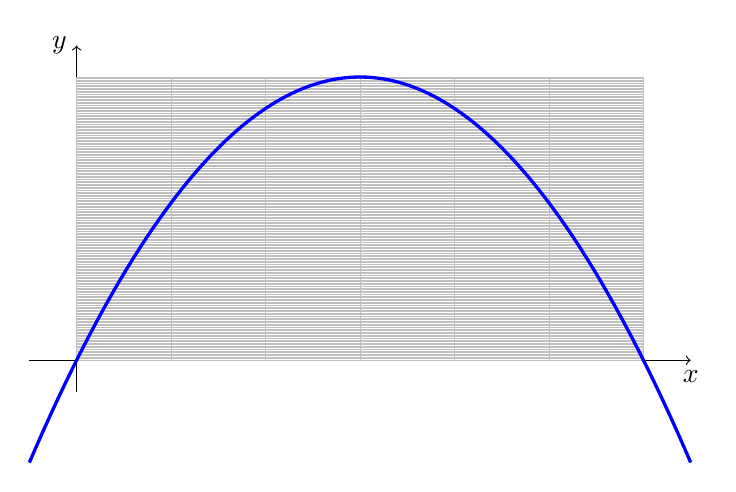
\begin{tikzpicture}[x=0.12cm, y=0.002cm]%
   % Scaling chosen so the vertex (30,1800) fits nicely:
   % 1 unit in x = 0.12 cm, 1 unit in y = 0.002 cm
   % Axes
   \draw[->] (-5,0) -- (65,0) node[below] {$x$};
   \draw[->] (0,-200) -- (0,2000) node[left] {$y$};

   % Grid (optional, light)
   \draw[step=10, very thin, lightgray] (0,0) grid (60,1800);

   % The curve y = 120x - 2x^2, drawn parametrically in x
   \draw[domain=-5:65, smooth, samples=300, very thick, blue]
     plot (\x, {120*\x - 2*\x*\x});

   % Intercepts
   %\fill (0,0) circle (1.2pt) node[below left] {$(0,0)$};
   %\fill (60,0) circle (1.2pt) node[below] {$(60,0)$};

   % Vertex
   %\fill (30,1800) circle (1.2pt) node[above right] {$(30,1800)$};

   % Dashed helper lines to the vertex (optional)
   %\draw[densely dashed, gray] (30,0) -- (30,1800);
   %\draw[densely dashed, gray] (0,1800) -- (30,1800);
 \end{tikzpicture}
        \end{image}
        %\xmalt{A graph of $y=120x-2x^2$.}
        \item What are the dimensions for the patch with the largest area, and what is this area?\\
        \textcolor{blue}{\[A(x)=x(120-2x)=120x-2x^2\]
        \[A'(x)=120-4x\]
        \[120-4x=0\]
        \[x=30\]
        The largest patch occurs when $x=30m$ and the length is $120-2(30)=60m$.  The area is $A(30)=30(60)=1800 m^2$}
    \end{enumerate}
\end{exercise}

\begin{exercise}
    A soup can in the shape of a right circular cylinder is made from two materials.  The material for the side of the can costs \$0.015 per square inch, and the material for the ends (lids) costs \$0.027 per square inch.  Suppose that we want to construct a can with a volume of 16 cubic inches.  What dimensions minimize the cost of the can? 
    \begin{enumerate}
        \item Draw a picture of the can and label its dimensions with appropriate variables.\\
          \begin{image}
            \includegraphics{optimization3A.png}
          \end{image}
          %\xmalt{A sketch of a right circular cylinder with height labelled $h$ and radius of the circle labelled $r$.}
        \item Use your variables to determine an expression for the volume, surface area, and cost of the can.\\
        \textcolor{blue}{Volume: $V=\pi r^2h$ \\
        Surface Area: $SA=2\pi r^2+2\pi rh$
        Cost: $C=0.027(2\pi r^2)+0.015(2\pi rh)$}\\
        \textcolor{orange}{The cost function and its relationship with the surface area function may not be obvious to all students.  Use their drawing as a way to help them make sense of it - in particular, help them break down the surface area formula if they are stuck.}
        \item Determine the total cost function as a function of a single variable.\\
        \textcolor{blue}{From the Volume equation we get that $h=\frac{V}{\pi r^2}$.  Since we know $V=16in^3$, we have that $h=\frac{16}{pi r^2}$.\\
        \[C=0.027(2\pi r^2)+0.015(2\pi r(\frac{16}{\pi r^2}))=0.027(2\pi r^2)+0.015(\frac{32}{r})=0.054\pi r^2+\frac{0.48}{r}\]
        \[C=0.054\pi r^2+\frac{0.48}{r}\]}\\
        \textcolor{orange}{It is conceivable that students may try to solve for $r$ instead of $h$.  It will be more painful to do it this way, so suggest they try with $h$, especially if they get stuck.}
        \item What is the domain on which you should consider this function?\\
        \textcolor{blue}{The radius cannot be negative, but can theoretically be any positive number or 0: $[0,\infty)$}
        \item Sketch the graph of the total cost function.  You may use a graphing calculator or Desmos. 
          \begin{image}
            \begin{tikzpicture}
  \begin{axis}[
    axis lines=middle,
    axis line style={-stealth},
    xlabel={$x$},
    ylabel={$y$},
    xmin=0, xmax=5,
    ymin=-5, ymax=25,
    samples=400,
    grid=both,
    minor tick num=1,
    tick align=outside,
    clip=false,
    every axis plot/.append style={thick, blue},
    legend style={draw=none, fill=none, at={(0.02,0.98)}, anchor=north west}
  ]

    % Plot for x > 0
    \addplot[
      domain=0.05:5
    ]
    {0.054*pi*x^2 + 0.48/x};

    \addlegendentry{$y = 0.054\pi x^2 + \dfrac{0.48}{x}$}

  \end{axis}
\end{tikzpicture}
          \end{image}
          %\xmalt{Graph of $y=0.054\pi x^2+\frac{0.48}{x}$ for $x>0$.}
        \item Find the absolute minimum cost and the dimensions that produce this value.\\
        \textcolor{blue}{\[C(r)=0.054\pi r^2+0.48r^{-1}\]
        \[C'(r)=0.108\pi r-0.48r^{-2}\]
        Find a common denominator: $C'(r)=\frac{0.108\pi r^3-0.48}{r^2}$\\
        If $C'(r)=0$, then the numerator must equal 0: $0.108\pi r^3-0.48=0$\\
        \[1.08\pi r^3=0.48\]\\
        \[r^3=1.415\]
        \[r\approx 1.123in\]\\
        Then $h=\frac{16}{\pi(1.123)^2}=4.038in$ and $C(1.123)=0.054\pi (1.123)^2+0.48(1.123)^{-1}\approx 0.64$ or 64 cents.} 
    \end{enumerate}
    Adapted from Boelkins, Austin \& Schlicker (2018) \textit{Active Calculus 2.1}.
\end{exercise}

\begin{exercise}
    Reflect on these problems.  What do they have in common and what is different?  What would you say to help someone who is going to solve these problems? \\
    This type of reflection can help you make connections and feel more confident when problems that don't look exactly the same as the problems you have done show up in other contexts.\\
    \textcolor{orange}{There is no correct answer to these questions.  These questions are here to help the students as they become more metacognitive in their approach to learning.}
\end{exercise}




\end{document}